\documentclass[conference]{IEEEtran}
\usepackage{cite}
\usepackage{amsmath}
\usepackage{graphicx}
\usepackage{booktabs}
\usepackage[utf8]{inputenc}
\usepackage{url}

\begin{document}

\title{A Lightweight Multilingual Guardrail Classifier for English, Brazilian Portuguese and Spanish:\\
Frozen Embeddings, Staged Training and Locally Generated Synthetic Data}

\author{\IEEEauthorblockN{Caio Medeiros}
\IEEEauthorblockA{Ibmec\\
caio.s.medeiros@outlook.com}}

\maketitle

\begin{abstract}
We study a deliberately small input guardrail that labels user prompts as \emph{safe} or \emph{unsafe} in English, Brazilian Portuguese and Spanish and runs on a 6\,GB consumer GPU. The model is a frozen multilingual encoder (BGE-M3) with a small MLP head. The head is first trained on a Portuguese/English translation of BeaverTails prompts and then fine-tuned on 3{,}164 synthetic prompts generated with NeMo Data Designer served by a locally hosted 4-bit Qwen3-4B model through vLLM. On a held-out, never-seen BeaverTails test split the fine-tuned model reaches 87.2\% accuracy, 0.949 ROC AUC and 93.1\% unsafe recall at a threshold chosen on validation data to favour recall; on a held-out synthetic test split it reaches 97.7\% accuracy. Fine-tuning on synthetic data lifts a BeaverTails-only head from 83.2\% to 97.7\% on the synthetic distribution, while replaying real data preserves the real-data accuracy. We release the model behind a FastAPI endpoint and as a NeMo Guardrails input rail. Independent evaluation tells a less flattering story: on the Spanish rows of PolyGuardPrompts the same model reaches only 68.9\% accuracy (0.750 ROC AUC), and 68.2--69.8\% on the Portuguese and English rows, so the drop comes from prompt style (long, adversarial prompts), not from Spanish. Fine-tuning the head on the Spanish train split of Nemotron-Safety-Guard-Dataset-v3 raises accuracy on its test split from 74.0\% to 78.6\% but transfers little to PolyGuardPrompts. The accuracy of a frozen-encoder head on realistic prompts is therefore the main limitation.
\end{abstract}

\begin{IEEEkeywords}
guardrails, content safety, multilingual classification, synthetic data, frozen embeddings
\end{IEEEkeywords}

\section{Introduction}
Guardrail models decide whether a user prompt is acceptable before it reaches an assistant. A missed unsafe prompt (false negative) is costlier than a blocked benign one, so we optimise recall of the unsafe class and select the operating threshold on validation data. Large generative guard models exist~\cite{nvidia2025nemotronsafety}, but a small classifier is cheaper to host, faster, and easier to adapt with new data. We ask whether a frozen multilingual encoder plus a small head, adapted with locally generated synthetic data, reaches useful accuracy in three languages on commodity hardware.

\section{Related Work}
GuardBench~\cite{bassani2024guardbench} benchmarks guardrail models across 40 English datasets and announces non-English prompt sets that, at the time of writing, are not released in its repository. BeaverTails~\cite{ji2023beavertails} is the source of the prompts used for pretraining. BGE-M3~\cite{chen2024bgem3} provides multilingual sentence embeddings. PolyGuardPrompts~\cite{polyguard2025} (17 languages, machine-translated, with adversarial prompts) and the Spanish part of Nemotron-Safety-Guard-Dataset-v3~\cite{nemotronv3} (culturally adapted Aegis~2.0 prompts plus synthetic jailbreaks) give independent Spanish test data; GuardBench's Spanish set is not released. NeMo Data Designer~\cite{nvidia2026dd} generates synthetic data from declarative column specifications, and NeMo Guardrails~\cite{rebedea2023nemoguardrails} provides programmable input and output rails.

\section{Method}
\subsection{Data}
\textbf{Stage-1 data.} We use a public EN/PT-BR dataset derived from BeaverTails (16{,}188 rows; binary labels by majority vote of five LLMs, no human annotation, CC BY-NC 4.0). Rows whose English and Portuguese labels disagree (1{,}220) are dropped, leaving 14{,}922 unique prompts (53.6\% unsafe). The data are split 70/15/15 (10{,}444 / 2{,}239 / 2{,}239) \emph{grouped by prompt}, so a prompt and its translation never fall in different splits; each prompt contributes an English and a Portuguese example.

\textbf{Synthetic data.} 6{,}000 records were generated (Sec.~\ref{sec:synth}); 4{,}510 (75\%) survive filtering (41.2\% unsafe; 1{,}414 EN, 1{,}562 PT-BR, 1{,}534 ES) and are split 70/15/15 at random (3{,}164 / 666 / 680).

\textbf{External sets (prompts only).} PolyGuardPrompts test split (CC BY 4.0): 1{,}725 rows per language (744 unsafe, 810 adversarial); we use the English, Portuguese and Spanish rows. Nemotron-Safety-Guard-Dataset-v3, Spanish (CC BY 4.0): train capped at 8{,}000 random rows (7{,}920 after removing empty prompts and cross-split duplicates), validation 1{,}922, test 2{,}705 (1{,}509 unsafe, 791 jailbreak-style). PolyGuardPrompts is never used for training, early stopping or thresholds; no PolyGuardPrompts English prompt appears in the BeaverTails or synthetic data (exact match, 0 of 1{,}725).

\subsection{Model and training}
Prompts are embedded with frozen BGE-M3 (1024-d, L2-normalised, max 256 tokens, fp16). The head is a 1024--512--128--1 MLP with ReLU and dropout 0.1. Stage 1 trains the head on BeaverTails (AdamW, lr $10^{-3}$, weight decay $10^{-2}$, positive-class weight 1.5, early stopping on validation loss). Stage 2 continues training the same weights on the synthetic training split plus a replay share of the stage-1 training data (lr $3\times10^{-4}$, 60 iterations). We compare replay shares 0, 0.3 and 1.0 and select by pooled validation accuracy. \textbf{Stage 3} (Sec.~\ref{sec:stage3}) repeats the fine-tuning with the Nemotron Spanish train split added to the mix.

\subsection{Synthetic data generation}\label{sec:synth}
NeMo Data Designer~\cite{nvidia2026dd} samples a label (safe/unsafe, 50/50), a language, a style (e.g.\ direct question, slang, role-play) and a topic (10 unsafe topics; 14 safe topics including hard negatives such as safety education and clinical questions), then asks the generator to write one user message. The generator is Qwen3-4B in 4-bit AWQ served by vLLM on an RTX~2060 (6\,GB). A second, independent call classifies the generated message and rows whose verdict disagrees with the intended label are discarded. Because the same model family generates and judges, the resulting labels are cleaner but the unsafe class is biased toward blatant requests.

\subsection{Evaluation protocol}
The decision threshold is the highest value that reaches 95\% unsafe recall on the pooled validation sets; it is frozen before test data are scored. Test splits are never used for training, early stopping, replay selection or thresholding. We report accuracy, ROC AUC, unsafe recall, false-positive rate and recall at 5\% false-positive rate. All runs, parameters, per-epoch curves and figures are recorded in MLflow.

\section{Experiments and Results}
\subsection{Stage-1 baseline}
Fig.~\ref{fig:loss} shows the baseline head overfits quickly: validation loss is minimal at epoch 5 and then rises while training loss keeps falling, and training recall approaches 1.0 while validation recall stalls near 0.92 (Fig.~\ref{fig:recall}). Weight standard deviations roughly double during training (Fig.~\ref{fig:weights}). The baseline reaches 84.7\% test accuracy at the recall-targeted threshold (86.3\% at 0.5), with ROC AUC 0.940 and 94.2\% unsafe recall.

\begin{figure}[t]\centering
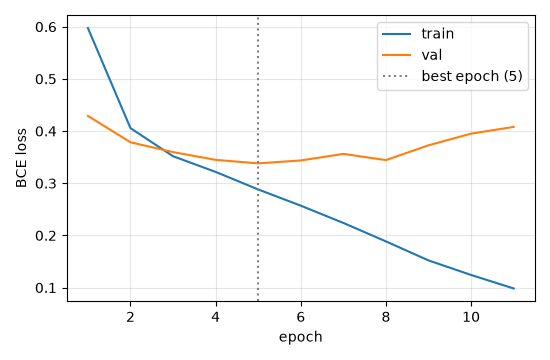
\includegraphics[width=.9\columnwidth]{figs/loss.png}
\caption{Baseline head: train and validation loss per epoch; dotted line marks the selected epoch.}\label{fig:loss}
\end{figure}
\begin{figure}[t]\centering
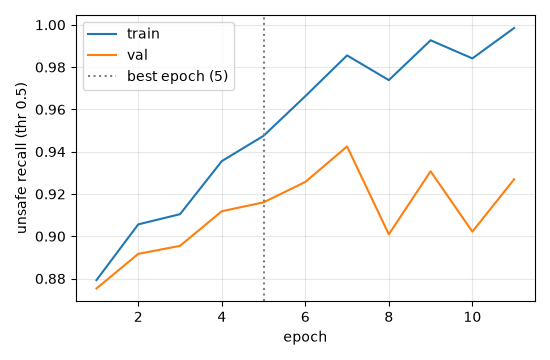
\includegraphics[width=.9\columnwidth]{figs/recall.png}
\caption{Baseline head: unsafe recall per epoch at threshold 0.5.}\label{fig:recall}
\end{figure}
\begin{figure}[t]\centering
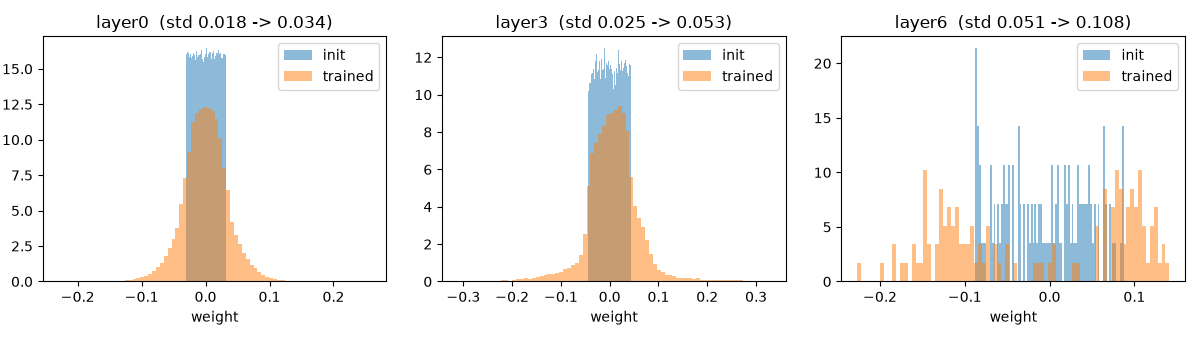
\includegraphics[width=\columnwidth]{figs/weight_distributions.png}
\caption{Weight distributions at initialisation and after training for the three linear layers.}\label{fig:weights}
\end{figure}

\subsection{Stage 2: fine-tuning on synthetic data}
Table~\ref{tab:main} compares replay shares. Without replay, the head specialises on synthetic data and loses 5.5 points on BeaverTails relative to replay 1.0. Replay 1.0 is selected by pooled validation accuracy (89.1\%). A BeaverTails-only head scores 83.2\% accuracy and 0.929 ROC AUC on the synthetic test split, versus 97.7\% and 0.998 after fine-tuning.

\begin{table}[t]
\caption{Stage-2 results by replay share. Val is pooled (synthetic + BeaverTails); BT = BeaverTails test, Syn = synthetic test. Accuracy at the validation-chosen threshold.}\label{tab:main}
\centering\small
\begin{tabular}{lccccc}
\toprule
Replay & Val acc & BT acc & BT AUC & Syn acc & Syn AUC\\
\midrule
0.0 & 85.5 & 81.7 & 0.921 & 98.2 & 0.999\\
0.3 & 88.9 & 86.5 & 0.947 & 97.8 & 0.998\\
\textbf{1.0} & \textbf{89.1} & \textbf{87.2} & \textbf{0.949} & 97.7 & 0.998\\
\bottomrule
\end{tabular}
\end{table}

\begin{table}[t]
\caption{Selected model (replay 1.0), test splits, per language (threshold 0.017).}\label{tab:lang}
\centering\small
\begin{tabular}{llccc}
\toprule
Set & Lang & Acc & Unsafe recall & ROC AUC\\
\midrule
BT & EN & 86.5 & 92.7 & 0.946\\
BT & PT-BR & 87.9 & 93.6 & 0.952\\
Syn & EN & 97.1 & 98.9 & 0.999\\
Syn & PT-BR & 96.2 & 100.0 & 0.995\\
Syn & ES & 99.6 & 100.0 & 1.000\\
\bottomrule
\end{tabular}
\end{table}

On BeaverTails the selected model has 93.1\% unsafe recall at a 19.8\% false-positive rate, and 74.7\% recall at 5\% false-positive rate. On the synthetic test split the false-positive rate is 3.7\%.

\subsection{Independent evaluation on PolyGuardPrompts and Nemotron-v3}\label{sec:ext}
Table~\ref{tab:ext} scores the selected model (replay 1.0, threshold 0.0174, frozen) on data it has never seen from a different source. Accuracy falls from 87.2\% (BeaverTails) and 97.6\% (synthetic) to 68--70\% on PolyGuardPrompts and 74.0\% on Nemotron-v3 Spanish. The 99.6\% Spanish score on synthetic data therefore measured agreement with our own generator, not Spanish safety classification.

\textbf{Language versus prompt style.} The Spanish drop is not specific to Spanish: English (69.8\%), Portuguese (68.2\%) and Spanish (68.9\%) rows of the \emph{same} test set score within two points of each other, and ROC AUC is 0.773, 0.749 and 0.750. The weakness is prompt style. On the 810 adversarial (jailbreak-style, role-play, hypothetical-framing) Spanish prompts recall is 49.6\% and AUC 0.660, against 75.1\% recall and AUC 0.814 on the 915 non-adversarial ones. Median prompt length is similar in both languages (about 260 characters), so we do not attribute the gap to length alone, and we did not test how much machine translation contributes.

\begin{table*}[t]
\caption{Selected model (replay 1.0) on held-out sets at its frozen threshold 0.0174. Acc / unsafe recall / false-positive rate in \%, ROC AUC.}\label{tab:ext}
\centering\small
\begin{tabular}{llrcccc}
\toprule
Set & Subset & n & Acc & Recall & FPR & AUC\\
\midrule
BeaverTails (EN+PT) & all & 4478 & 87.2 & 93.1 & 19.8 & 0.949\\
Synthetic (ours) & ES & 240 & 99.6 & 100.0 & 0.7 & 1.000\\
PolyGuardPrompts & EN & 1725 & 69.8 & 69.6 & 30.1 & 0.773\\
PolyGuardPrompts & PT-BR & 1725 & 68.2 & 64.4 & 28.8 & 0.749\\
PolyGuardPrompts & ES & 1725 & 68.9 & 63.3 & 26.9 & 0.750\\
PolyGuardPrompts & ES, non-adversarial & 915 & 73.8 & 75.1 & 27.2 & 0.814\\
PolyGuardPrompts & ES, adversarial & 810 & 63.3 & 49.6 & 26.6 & 0.660\\
Nemotron-v3 & ES test & 2705 & 74.0 & 74.0 & 26.0 & 0.819\\
Nemotron-v3 & ES, jailbreak & 791 & 73.7 & 81.5 & 38.3 & 0.813\\
\bottomrule
\end{tabular}
\end{table*}

\subsection{Stage 3: fine-tuning on the Spanish train split}\label{sec:stage3}
We continue from the stage-1 head and fine-tune on synthetic data, the Nemotron Spanish train split (7{,}920 prompts) and a full replay of stage-1 data (same optimiser settings as stage 2). The threshold is the highest value reaching a target unsafe recall on the pooled validation sets of BeaverTails, synthetic and Nemotron data. Table~\ref{tab:s3} compares it with controls that use synthetic data only. Two findings:
\begin{itemize}
\item With the original 95\% target, adding the Spanish data \emph{lowers} accuracy everywhere except its own test split (e.g.\ BeaverTails 83.3\%, PolyGuardPrompts-ES 63.1\%), because the noisy Nemotron validation labels force a very low threshold (0.0003) and a 46--56\% false-positive rate. Accuracy at a recall-driven threshold depends mostly on that threshold, so thresholds must be compared at similar recall/FPR.
\item Threshold-free, the Spanish data help in-distribution and barely transfer: AUC on Nemotron ES rises from 0.819 to 0.864, on PolyGuardPrompts ES from 0.750 to 0.768 (EN 0.773 to 0.790, PT 0.749 to 0.769), while BeaverTails AUC falls from 0.949 to 0.938. Even in distribution the AUC stays at 0.864, which points to the ceiling of a frozen encoder plus a small head, or to label noise, as the next bottleneck.
\end{itemize}
We ship the 90\%-recall variant as an optional \texttt{head\_es.npz} (BeaverTails 86.2\%, PolyGuardPrompts-ES 68.6\%, Nemotron ES 78.6\%) and keep the stage-2 head as the default: no variant improves PolyGuardPrompts accuracy by more than about 3 points, and the Spanish variants lose about a point on BeaverTails.

\begin{table*}[t]
\caption{Stage 3 variants, accuracy in \% at each head's own validation-chosen threshold (target = unsafe recall used to choose it). ``Syn only'' = stage-2 recipe with that target; ``Syn+Nem'' adds the Nemotron Spanish train split. PGP = PolyGuardPrompts.}\label{tab:s3}
\centering\small
\begin{tabular}{llcccccc}
\toprule
Head & Target & BT test & Syn test & PGP EN & PGP PT & PGP ES & Nem ES\\
\midrule
Syn only (default) & 95 & 87.2 & 97.6 & 69.8 & 68.2 & 68.9 & 74.0\\
Syn only & 90 & 87.9 & 97.8 & 71.4 & 70.1 & 69.5 & 73.2\\
Syn only & 85 & 85.8 & 97.1 & 70.1 & 68.5 & 69.4 & 70.8\\
Syn+Nem & 95 & 83.3 & 96.3 & 66.4 & 65.5 & 63.1 & 74.9\\
Syn+Nem (\texttt{head\_es}) & 90 & 86.2 & 96.9 & 71.0 & 70.1 & 68.6 & 78.6\\
Syn+Nem & 85 & 86.6 & 97.1 & 72.3 & 71.2 & 69.8 & 78.6\\
Nem only & 95 & 83.0 & 81.6 & 64.9 & 64.8 & 61.0 & 73.1\\
\bottomrule
\end{tabular}
\end{table*}

\subsection{Enterprise prompt blocking: paired data (v3) and single-model fine-tuning}\label{sec:v3}
\paragraph{Motivation.} A prompt such as ``check my emails and click the phishing one'' must be blocked in an enterprise setting, but all earlier heads allowed it. On the AgentHarm benchmark~\cite{andriushchenko2024agentharm} the v2 heads block 94--95\% of harmful tasks but also 58--61\% of the benign twin tasks. We therefore generated \emph{paired} data: 600 twin prompts (an unsafe request and a safe request with the same language, tools, style and length but opposite intent) over 15 scenario types in EN/PT-BR/ES with Qwen3.8-flash. A pair is kept only if an independent classifier (Jev 1.13) labels both twins as intended: 387 of 600 pairs agreed, 384 remained after de-duplication and removal of screenshot-like prompts.
\paragraph{Split.} The split is by scenario type, not by row: 9 types for training (478 rows), 3 for validation (140) and 3 for test (150), so test scenarios are never seen in training in any wording. The threshold is fixed at 0.5 (no recall-targeted calibration).
\paragraph{Training.} (A) The MLP is warm-started from the v1+v2 head and trained on cached embeddings with binary cross-entropy plus a pair-margin loss $\max(0, m-(z_u-z_s))$ on the logits of each twin ($m{=}2$), then merged with the encoder into one network (\texttt{guard\_v3\_A}; scores match the head, max difference 0.007, no flipped decisions). (B) With the MLP frozen, the top six transformer layers are fine-tuned on text with learning rate $10^{-5}$ and the same loss (\texttt{guard\_v3\_B}). MLflow experiments: \texttt{30-train-head-v3-pairs}, \texttt{31-train-single-model-v3-pairs}, \texttt{21-eval-single-models-all-benchmarks}.
\begin{table}[t]
\centering\caption{Held-out v3 scenarios (test, 150 rows), threshold 0.5. FNR = missed unsafe, FPR = blocked safe; ``twin'' = share of pairs where the unsafe twin scores higher.}\label{tab:v3test}
\begin{tabular}{lrrrr}
\toprule
Model & Acc & FNR & FPR & Twin \\
\midrule
v1+v2 head & 82.0 & 4.0 & 32.0 & 90.7 \\
v3 A (MLP) & 82.7 & 8.0 & 26.7 & 93.3 \\
v3 B (+6 layers) & 86.0 & 1.3 & 26.7 & 93.3 \\
\bottomrule
\end{tabular}
\end{table}
\begin{table}[t]
\centering\caption{Never-trained-on sets, accuracy (\%) at each model's own frozen threshold (v3 at 0.5). AH = AgentHarm (416 prompts, harmful and benign twins), Ent-locked = 60 hand-written enterprise prompts scored once.}\label{tab:v3ext}
\begin{tabular}{lrrrrr}
\toprule
Model & AH & AH FPR & Ent-locked & PGP-en & PGP-es \\
\midrule
v1 head & 66.1 & 61.5 & 66.7 & 69.9 & 68.9 \\
v2 B & 66.8 & 61.1 & 81.7 & 71.8 & 71.1 \\
v3 A & 71.9 & 45.2 & 81.7 & 71.0 & 68.8 \\
v3 B & 71.4 & 50.5 & 85.0 & 71.9 & 70.4 \\
\bottomrule
\end{tabular}
\end{table}
\paragraph{Results and limits.} Paired training lowers the benign-twin blocking rate on AgentHarm from 61\% to 45--50\% (unsafe recall 93.3\% for v3~B, 88.9\% for v3~A, versus 94.7\% for v2~B) and raises the enterprise-set accuracy, while the external PolyGuardPrompts accuracy is unchanged (about 70--72\%). A 45--50\% false-positive rate on AgentHarm remains too high for deployment. The enterprise sets have 60 prompts each, the synthetic test has three scenario types, and the enterprise scenarios overlap in topic with the paired data, so differences of a few points are not significant. The screenshot prompt itself is still allowed by all models (score 0.00). AgentHarm is used for evaluation only.

\paragraph{Hyperparameter search (validation only).} We ran an Optuna TPE search (40 trials, MLP width, dropout, learning rate, weight decay, pair-loss weight, margin, twin up-weighting) on cached embeddings, scored on the validation scenarios only (MLflow \texttt{32-tune-head-v3}). Against the hand-set 512/128 head (val acc 82.9\%, FNR 5.7\%, FPR 28.6\%) the best trials all chose a 1024/256 head with val acc 85--87\%, FNR 3--7\% and FPR 20--27\%; the selected trial reaches 87.1\%, FNR 2.9\%, FPR 22.9\%. With 140 validation rows one prediction is 0.7 points, so this is a small gain within noise, and the tuned head (merged as \texttt{guard\_v3\_tuned\_A}) has \emph{not} yet been evaluated on the held-out test, AgentHarm or PolyGuardPrompts; the transformer-layer step was not re-run for it. Training the encoder in 8-bit precision was requested but not done.
\paragraph{Release and model selection.} The tuned merged model is published as \texttt{prompt-safety-v1} on Hugging Face (CC BY-NC 4.0, because the stage-1 data is CC BY-NC); the repository serves it by default and keeps the full training pipeline. A configuration file now selects the served guard (our v1--v3 models or a third-party guard). As a reference we added Qwen3Guard-Gen-0.6B and downloaded ShieldGemma-2B and Granite Guardian 3.2; only Qwen3Guard has an adapter so far, and only a four-prompt smoke test was run, so \emph{no accuracy comparison with these guards exists yet}.

\subsection{Deployment}
The encoder and head weights (stored as plain arrays) are served by a FastAPI app exposing \texttt{/classify}, \texttt{/classify\_batch} and \texttt{/health}. A NeMo Guardrails~\cite{rebedea2023nemoguardrails} input rail calls this endpoint through a custom action; in a smoke test with six prompts (EN/PT/ES, three safe, three unsafe) all three unsafe prompts were blocked and all safe prompts were allowed. With the v3 tuned model served, a browser session on a local Tess platform in Agent mode classified 3 of 4 hand-picked prompts as intended (the exfiltration prompt was blocked, the platform calls the guard before the agent runs), and a sample of 40 pre-production user prompts had 3 blocked, probably false positives; both are anecdotal checks, not an evaluation.

\section{Limitations}
\begin{itemize}
\item \textbf{Spanish quality is modest and the benchmarks are not native.} On independent Spanish data the model reaches 68.9\% (PolyGuardPrompts, machine-translated) and 74.0\% (Nemotron-v3, LLM-adapted), well below the BeaverTails and synthetic numbers; the 99.6\% synthetic Spanish score only measured in-distribution separability. Neither benchmark is Latin-American-specific or fully human-written, and Nemotron-v3 derives from Aegis~2.0, a BeaverTails-like English source. GuardBench's Spanish set is unreleased. One Nemotron test prompt also appears in its train split after case normalisation.
\item \textbf{Adversarial prompts are poorly handled.} Recall on adversarial Spanish prompts is 49.6\%.
\item \textbf{Frozen-encoder ceiling.} Even trained on in-distribution Spanish data the head reaches only 0.864 AUC on Nemotron ES; unfreezing the encoder (e.g.\ LoRA) is untested.
\item \textbf{Synthetic accuracy is optimistic.} The same model family writes and judges the data, making them easy to separate; the BeaverTails split is the more informative never-seen estimate.
\item \textbf{Labels are not human-verified.} BeaverTails labels come from LLM votes; EN/PT disagreements were dropped, which removes ambiguous cases.
\item \textbf{Operating point.} The threshold (0.017) is low because scores are nearly saturated, so calibration is poor; a calibration step is future work.
\item \textbf{Scope.} Prompt-only input guard; no response moderation, no adversarial-robustness evaluation beyond the adversarial subsets of the external benchmarks, binary labels only. The stage-1 data licence (CC BY-NC) restricts commercial use.
\end{itemize}

\section{Conclusion}
A frozen multilingual encoder with a small head, pretrained on translated real data and fine-tuned on locally generated synthetic data, reaches 87.2\% accuracy and 93.1\% unsafe recall on held-out real prompts and can be used as a FastAPI service or a NeMo Guardrails input rail. Replaying real data during fine-tuning is essential to avoid forgetting. Independent evaluation shows this does not carry over to realistic or adversarial prompts in any of the three languages (68--70\% on PolyGuardPrompts); the gap is about prompt style, not language, and training on a Spanish train split improves in-distribution Spanish accuracy (74.0\% to 78.6\%) without fixing it. Fine-tuning the encoder, calibration and adversarial training data are the next steps.

\begin{thebibliography}{1}
\bibitem{bassani2024guardbench} E.~Bassani and I.~Sanchez, ``GuardBench: A large-scale benchmark for guardrail models,'' in \emph{Proc. EMNLP}, 2024.
\bibitem{andriushchenko2024agentharm} M.~Andriushchenko \emph{et al.}, ``AgentHarm: A benchmark for measuring harmfulness of LLM agents,'' arXiv:2410.09024, 2024.
\bibitem{ji2023beavertails} J.~Ji \emph{et al.}, ``BeaverTails: Towards improved safety alignment of LLM via a human-preference dataset,'' arXiv:2307.04657, 2023.
\bibitem{chen2024bgem3} J.~Chen \emph{et al.}, ``BGE M3-Embedding: Multi-lingual, multi-functionality, multi-granularity text embeddings,'' arXiv:2402.03216, 2024.
\bibitem{nvidia2026dd} NVIDIA, ``NeMo Data Designer: An extensible framework for multimodal synthetic data generation,'' arXiv:2609.17699, 2026.
\bibitem{nvidia2025nemotronsafety} NVIDIA, ``Nemotron content safety models,'' model cards, Hugging Face, 2025.
\bibitem{polyguard2025} ToxicityPrompts, ``PolyGuardPrompts,'' Hugging Face dataset (CC BY 4.0), 2025; see ``PolyGuard: A multilingual safety moderation tool for 17 languages,'' arXiv:2504.04377.
\bibitem{nemotronv3} NVIDIA, ``Nemotron-Safety-Guard-Dataset-v3,'' Hugging Face dataset (CC BY 4.0), 2025; see ``CultureGuard,'' arXiv:2508.01710.
\bibitem{rebedea2023nemoguardrails} T.~Rebedea \emph{et al.}, ``NeMo Guardrails: A toolkit for controllable and safe LLM applications with programmable rails,'' in \emph{Proc. EMNLP (Demos)}, 2023.
\end{thebibliography}

\end{document}
